% -*- latex -*-
%%%%%%%%%%%%%%%%%%%%%%%%%%%%%%%%%%%%%%%%%%%%%%%%%%%%%%%%%%%%%%%%
%%%%%%%%%%%%%%%%%%%%%%%%%%%%%%%%%%%%%%%%%%%%%%%%%%%%%%%%%%%%%%%%
%%%%
%%%% This text file is part of the source of 
%%%% `Introduction to High-Performance Scientific Computing'
%%%% by Victor Eijkhout, copyright 2012-7
%%%%
%%%% This book is distributed under a Creative Commons Attribution 3.0
%%%% Unported (CC BY 3.0) license and made possible by funding from
%%%% The Saylor Foundation \url{http://www.saylor.org}.
%%%%
%%%%%%%%%%%%%%%%%%%%%%%%%%%%%%%%%%%%%%%%%%%%%%%%%%%%%%%%%%%%%%%%
%%%%%%%%%%%%%%%%%%%%%%%%%%%%%%%%%%%%%%%%%%%%%%%%%%%%%%%%%%%%%%%%

\Level 1 {Goto matrix-matrix product}
\label{sec:goto-gemm}
\index{matrix!matrix product!Goto implementation|(textbf}

In section~\ref{sec:gemm} we argued that the \indexterm{matrix-matrix
product} (or \indextermtt{dgemm} in \indexac{BLAS} terms) has a large amount of
possible data reuse: there are $O(n^3)$ operations on $O(n^2)$ data.
We will now consider an implementation, due
to \indextermsub{Kazushige}{Goto}~\cite{GotoGeijn:2008:Anatomy}, that
indeed achieves close to peak performance.

The matrix-matrix algorithm has three loops, each of which we can block,
giving a six-way nested loop.
Since there are no recurrences on the output elements, all resulting
loop exchanges are legal. Combine this with the fact that the loop blocking
introduces three blocking parameters, and you'll see that the number of
potential implementations is enormous. Here we present the global reasoning
that underlies the Goto implementation; for a detailed discussion see the paper cited.

We start by writing the product $C\leftarrow A\cdot B$ (or
  $C\leftarrow C+AB$ according to the Blas standard) as a sequence of
  low-rank updates:
\[ C_{**} = \sum_k  A_{*k}B_{k*} \]
\begin{figure}[ht]

\includegraphics[scale=.1]{gotoblas1}
\caption{Matrix-matrix multiplication as a sequence of low-rank updates}
\label{fig:goto1}
\end{figure}
See figure~\ref{fig:goto1}. Next we derive the `block-panel' multiplication
by multiplying a block of~$A$ by a `sliver' of~$B$; see figure~\ref{fig:goto2}.
\begin{figure}[ht]
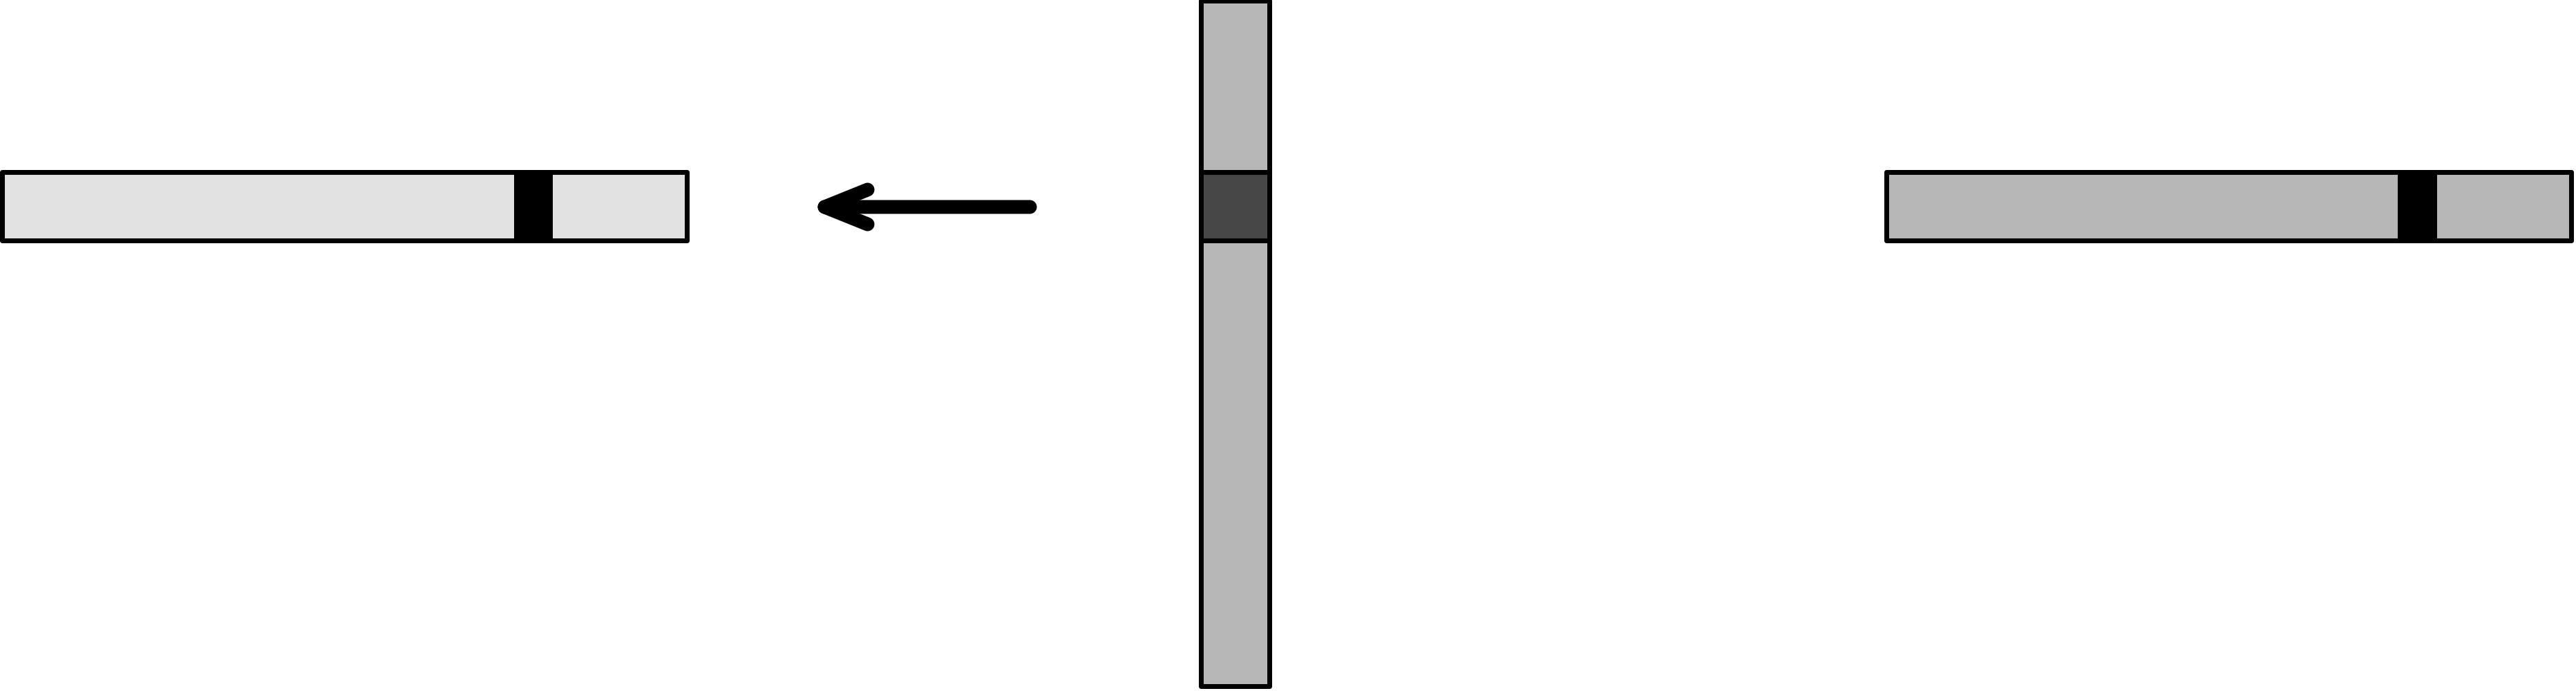
\includegraphics[scale=.1]{gotoblas2}  
\caption{The block-panel multiplication in the matrix-matrix algorithm}
\label{fig:goto2}
\end{figure}
Finally, the inner algorithm accumulates a small row $C_{i,*}$,
typically of small size such as~4, by accumulating:
\begin{verbatim}
// compute C[i,*] :
for k:
   C[i,*] = A[i,k] * B[k,*]
\end{verbatim}
See figure~\ref{fig:goto3}.
\begin{figure}[ht]
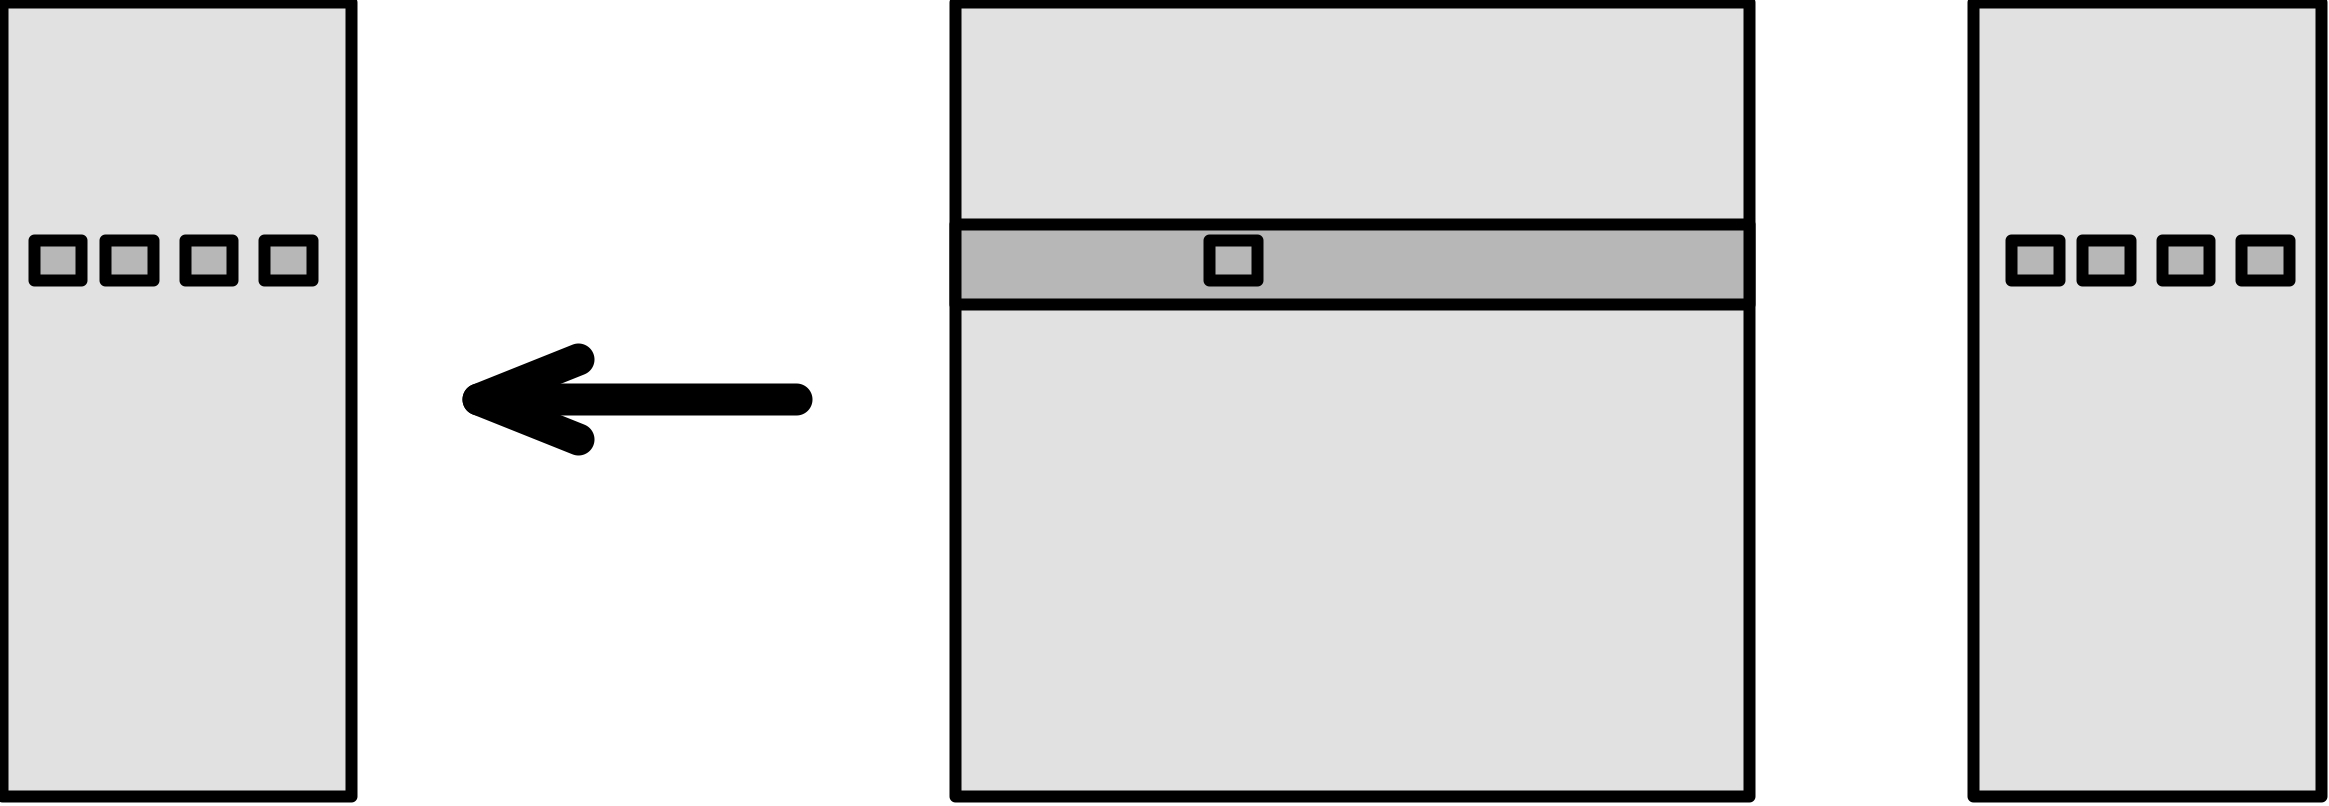
\includegraphics[scale=.12]{gotoblas3}
\caption{The register-resident kernel of the matrix-matrix multiply}
\label{fig:goto3}
\end{figure}
Now this algorithm is tuned.
\begin{itemize}
\item We need enough registers for \verb+C[i,*]+, \verb+A[i,k]+ and
  \verb+B[k,*]+. On current processors that means that we accumulate
  four elements of~$C$.
\item Those elements of~$C$ are accumulated, so they stay in register
  and the only data transfer is loading of the elements of $A$
  and~$B$; there are no stores!
\item The elements \verb+A[i,k]+ and \verb+B[k,*]+ stream from L1.
\item Since the same block of~$A$ is used for many successive slivers
  of~$B$, we want it to stay resident; we choose the blocksize of $A$
  to let it stay in L2 cache.
\item In order to prevent TLB problems, $A$~is stored by rows. If we
  start out with a matrix in (Fortran) \indexterm{column-major}
  storage, this means we have to make a copy. Since copying is of a
  lower order of complexity, this cost is amortizable.
\end{itemize}

This algorithm be implemented in specialized hardware, as in the
\indextermbus{Google}{TPU}~\cite{GoogleTPUpage}, giving great energy efficiency.

\index{matrix-matrix product!Goto implementation|)}

\begin{comment}
\begin{verbatim}
int l1size,l2size, i1,i2, n1,n2;
double *data; int savedptr, ptr = 0;

save2 = 0;
for (i2=0; i2<n2; i2++) {
  save1 = save2;
  for (i1=0; i1<n1; i1++) {
    ptr = save1;
    for ( ; ptr<save1+l1size; ) {
      ..... = .... data[ptr++] ....
    }
    if (i1%3==1) save1 += l1size;
  }
  if (i2%2==1) save2 += l2size;
}
\end{verbatim}
\end{comment}

\index{matrix!matrix product!Goto implementation|)}

